\documentclass[12pt]{article}
\usepackage{amsmath}
\usepackage{latexsym}
\usepackage{amsfonts}
\usepackage[normalem]{ulem}
\usepackage{soul}
\usepackage{array}
\usepackage{amssymb}
\usepackage{extarrows}
\usepackage{graphicx}
\usepackage[backend=biber,
style=numeric,
sorting=none,
isbn=false,
doi=false,
url=false,
]{biblatex}\addbibresource{bibliography.bib}

\usepackage{subfig}
\usepackage{wrapfig}
\usepackage{wasysym}
\usepackage{enumitem}
\usepackage{adjustbox}
\usepackage{ragged2e}
\usepackage[svgnames,table]{xcolor}
\usepackage{tikz}
\usepackage{longtable}
\usepackage{changepage}
\usepackage{setspace}
\usepackage{hhline}
\usepackage{multicol}
\usepackage{tabto}
\usepackage{float}
\usepackage{multirow}
\usepackage{makecell}
\usepackage{fancyhdr}
\usepackage[toc,page]{appendix}
\usepackage[hidelinks]{hyperref}
\usetikzlibrary{shapes.symbols,shapes.geometric,shadows,arrows.meta}
\tikzset{>={Latex[width=1.5mm,length=2mm]}}
\usepackage{flowchart}\usepackage[paperheight=11.69in,paperwidth=8.27in,left=1.0in,right=1.0in,top=1.0in,bottom=1.0in,headheight=1in]{geometry}
\usepackage[utf8]{inputenc}
\usepackage[T1]{fontenc}
\TabPositions{0.5in,1.0in,1.5in,2.0in,2.5in,3.0in,3.5in,4.0in,4.5in,5.0in,5.5in,6.0in,}

\urlstyle{same}


 %%%%%%%%%%%%  Set Depths for Sections  %%%%%%%%%%%%%%

% 1) Section
% 1.1) SubSection
% 1.1.1) SubSubSection
% 1.1.1.1) Paragraph
% 1.1.1.1.1) Subparagraph


\setcounter{tocdepth}{5}
\setcounter{secnumdepth}{5}


 %%%%%%%%%%%%  Set Depths for Nested Lists created by \begin{enumerate}  %%%%%%%%%%%%%%


\setlistdepth{9}
\renewlist{enumerate}{enumerate}{9}
		\setlist[enumerate,1]{label=\arabic*)}
		\setlist[enumerate,2]{label=\alph*)}
		\setlist[enumerate,3]{label=(\roman*)}
		\setlist[enumerate,4]{label=(\arabic*)}
		\setlist[enumerate,5]{label=(\Alph*)}
		\setlist[enumerate,6]{label=(\Roman*)}
		\setlist[enumerate,7]{label=\arabic*}
		\setlist[enumerate,8]{label=\alph*}
		\setlist[enumerate,9]{label=\roman*}

\renewlist{itemize}{itemize}{9}
		\setlist[itemize]{label=$\cdot$}
		\setlist[itemize,1]{label=\textbullet}
		\setlist[itemize,2]{label=$\circ$}
		\setlist[itemize,3]{label=$\ast$}
		\setlist[itemize,4]{label=$\dagger$}
		\setlist[itemize,5]{label=$\triangleright$}
		\setlist[itemize,6]{label=$\bigstar$}
		\setlist[itemize,7]{label=$\blacklozenge$}
		\setlist[itemize,8]{label=$\prime$}

\setlength{\topsep}{0pt}\setlength{\parindent}{0pt}

 %%%%%%%%%%%%  This sets linespacing (verticle gap between Lines) Default=1 %%%%%%%%%%%%%%


\renewcommand{\arraystretch}{1.3}


%%%%%%%%%%%%%%%%%%%% Document code starts here %%%%%%%%%%%%%%%%%%%%



\begin{document}
\begin{Center}
Algoritmos de encriptación
\end{Center}\par


\vspace{\baselineskip}
\begin{Center}
Cristian Guzmán Rivera
\end{Center}\par


\vspace{\baselineskip}
\begin{Center}
Ingeniería de Sistemas - Diseño de Algoritmos
\end{Center}\par

\begin{Center}
\\
Noviembre 2019
\end{Center}\par


\vspace{\baselineskip}

\vspace{\baselineskip}
\begin{Center}
\textbf{Introducción}
\end{Center}\par


\vspace{\baselineskip}
\begin{justify}
El cifrado de datos y el uso de algoritmos de encriptación son fundamentales para la seguridad de un Sistema de Control de Accesos, ya que garantizan la invulnerabilidad de las comunicaciones entre los dispositivos que lo componen.
\end{justify}\par


\vspace{\baselineskip}
\begin{justify}
Su uso es imprescindible para evitar ataques al sistema, ya que permiten que la información que se intercambia entre los distintos elementos sea totalmente indescifrable para usuarios ajenos al mismo.
\end{justify}\par


\vspace{\baselineskip}
\begin{Center}
\textbf{Algoritmos Simétricos}
\end{Center}\par


\vspace{\baselineskip}
\begin{justify}
El cifrado mediante clave simétrica significa que dos o más usuarios, tienen una única clave secreta, esta clave será la que cifrará y descifrará la información transmitida a través del canal inseguro.\textbf{ }
\end{justify}\par


\vspace{\baselineskip}
\begin{justify}
Es decir, la clave secreta la debe tener los dos usuarios, y con dicha clave, el usuario A cifrará la información, la mandará a través del canal inseguro, y a continuación el usuario B descifrará esa información con la MISMA clave que ha usado el usuario A.
\end{justify}\par


\vspace{\baselineskip}
\begin{justify}
Para que un algoritmo de clave simétrica sea fiable debe cumplir:
\end{justify}\par


\vspace{\baselineskip}
\begin{justify}
– Una vez que el mensaje es cifrado, no se puede obtener la clave de cifrado/descifrado ni tampoco el texto en claro.
\end{justify}\par

\begin{justify}
– Si conocemos el texto en claro y el cifrado, se debe tardar más y gastar más dinero en obtener la clave, que el posible valor derivado de la información sustraída (texto en claro).
\end{justify}\par


\vspace{\baselineskip}
\begin{justify}
Ya sabiendo todo eso, estos son algunos de los algoritmos simétricos son:
\end{justify}\par


\vspace{\baselineskip}
\begin{justify}
\textbf{DES (DATA ENCRYPTION STANDARD)} 
\end{justify}\par


\vspace{\baselineskip}
\begin{justify}
Este algoritmo de cifrado aplica sucesivas permutaciones y sustituciones al texto en claro. En un primer momento la información de 64bits se somete a una permutación inicial, y a continuación se somete a una permutación con entrada de 8 bits, y otra de sustitución de entrada de 5 bits, todo ello constituido a través de un proceso con 16 etapas de cifrado.
\end{justify}\par


\vspace{\baselineskip}
\begin{justify}
El algoritmo DES usa una clave simétrica de 64 bits, los 56 primeros bits son empleados para el cifrado, y los 8 bits restantes se usan para comprobación de errores durante el proceso. La clave efectiva es de 56 bits, por tanto, tenemos 2⁵⁶ combinaciones posibles, por lo que la fuerza bruta se hace casi imposible.
\end{justify}\par


\vspace{\baselineskip}
\begin{justify}
Ventajas
\end{justify}\par

\begin{justify}
– Es uno de los sistemas más empleados y extendidos, por tanto es de los más probados.
\end{justify}\par

\begin{justify}
– Implementación sencilla y rápida.
\end{justify}\par


\vspace{\baselineskip}
\begin{justify}
Inconvenientes
\end{justify}\par

\begin{justify}
– No se permite una clave de longitud variable, es decir, no se puede aumentar para tener una mayor seguridad.
\end{justify}\par

\begin{justify}
– Es vulnerable al criptoanálisis diferencial (2⁴⁷ posibilidades) siempre que se conozco un número suficiente de textos en claro y cifrados.
\end{justify}\par

\begin{justify}
– La longitud de clave de 56 bits es demasiado corta, y por tanto vulnerable. Actualmente DES ya no es un estándar, debido a que en 1999 fue roto por un ordenador.
\end{justify}\par


\vspace{\baselineskip}
\begin{justify}
\textbf{3DES (TRIPLE DATA ENCRYPTION STANDARD)}
\end{justify}\par


\vspace{\baselineskip}
\begin{justify}
Se basa en aplicar el algoritmo DES tres veces, la clave tiene una longitud de 128 bits. Si se cifra el mismo bloque de datos dos veces con dos llaves diferentes (de 64 bits), aumenta el tamaño de la clave.
\end{justify}\par


\vspace{\baselineskip}
\begin{justify}
El 3DES parte de una llave de 128 bits, que es divida en dos llaves, A y B.
\end{justify}\par


\vspace{\baselineskip}
\begin{justify}
Al recibir los datos, aplicamos el algoritmo DES con la llave A, a continuación se repite con la llave B y luego otra vez con la llave A (de nuevo).
\end{justify}\par


\vspace{\baselineskip}
\begin{justify}
3DES aumenta de forma significativa la seguridad del sistema de DES, pero requiere más recursos del ordenador.
\end{justify}\par


\vspace{\baselineskip}
\begin{justify}
\textbf{RC4}
\end{justify}\par


\vspace{\baselineskip}
\begin{justify}
RC4 es un algoritmo de cifrado de flujo diseñado por Ron Rivest para RSA Data Security. Es un algoritmo de tamaño de clave variable con operaciones a nivel de byte. Es un algoritmo de ejecución rápida en software. El algoritmo se emplea para encriptación de ficheros y para encriptar la comunicación en protocolos como el SSL (TLS).
\end{justify}\par


\vspace{\baselineskip}
\begin{justify}
\textbf{RC5}
\end{justify}\par


\vspace{\baselineskip}
\begin{justify}
Se aplican operaciones XOR sobre los datos, pudiendo ser de 32, 64 o 128 bits. Permite diferentes longitudes de clave, y un número variable de iteraciones (la seguridad del cifrado aumenta exponencialmente cuanto mayor número de iteraciones), también funciona como un generador de número aleatorios, sumándoles a los bloques de texto rotados mediante la XOR.
\end{justify}\par


\vspace{\baselineskip}
\begin{justify}
\textbf{IDEA (INTERNATIONAL DATA ENCRIPTION ALGORITHM)}
\end{justify}\par


\vspace{\baselineskip}
\begin{justify}
Aplica una clave de 128 bits sin paridad a bloques de datos de 64 bits, y se usa tanto para cifrar como para descifrar.
\end{justify}\par


\vspace{\baselineskip}
\begin{justify}
Se alteran los datos de entrada en una secuencia de iteraciones parametrizadas, con el objetivo de producir bloques de salida de texto cifrado de 64 bits. IDEA combina operaciones matemáticas como XOR, sumas con acarreo de módulo 2¹⁶ y multiplicaciones de módulo 2¹⁶+1, sobre bloques de 16 bits.
\end{justify}\par


\vspace{\baselineskip}
\begin{justify}
\textbf{AES (ADVANCED ENCRYPTION STANDARD)}
\end{justify}\par


\vspace{\baselineskip}
\begin{justify}
Este algoritmo es el más conocido entre los usuarios de routers, ya que WPA opera con AES como método de cifrado. Este cifrado puede implementar tanto en sistemas hardware como en software. El sistema criptográfico AES opera con bloques y claves de longitudes variable, hay AES de 128 bits, de 192 bits y de 256 bits.
\end{justify}\par


\vspace{\baselineskip}
\begin{justify}
El resultado intermedio del cifrado constituye una matriz de bytes de cuatro filas por cuatro columnas. A esta matriz se le vuelve a aplicar una serie de bucles de cifrado basado en operaciones matemáticas (sustituciones no lineales de bytes, desplazamiento de filas de la matriz, combinaciones de las columnas mediante multiplicaciones lógicas y sumas XOR en base a claves.
\end{justify}\par


\vspace{\baselineskip}


%%%%%%%%%%%%%%%%%%%% Figure/Image No: 1 starts here %%%%%%%%%%%%%%%%%%%%

\begin{figure}[H]
	\begin{Center}
		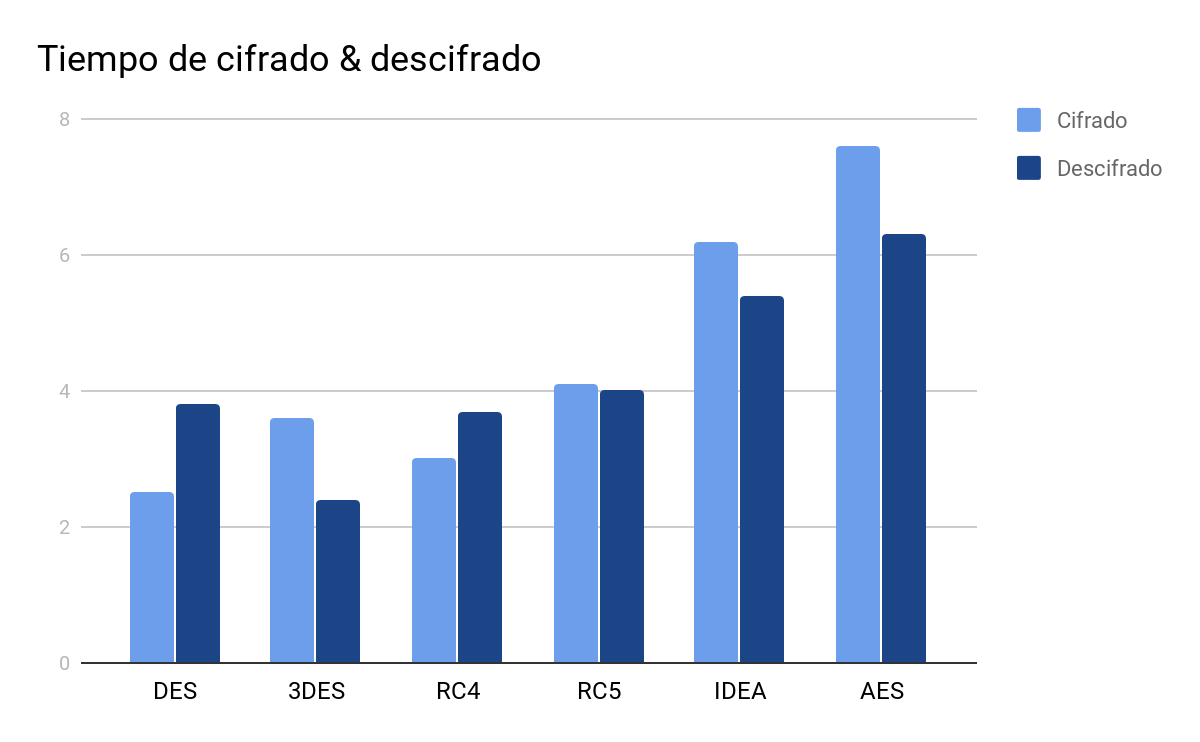
\includegraphics[width=6.27in,height=3.88in]{./media/image2.png}
	\end{Center}
\end{figure}


%%%%%%%%%%%%%%%%%%%% Figure/Image No: 1 Ends here %%%%%%%%%%%%%%%%%%%%

\par


\vspace{\baselineskip}
\begin{Center}
\textbf{Encriptación Asimétrica}
\end{Center}\par


\vspace{\baselineskip}
\begin{justify}
La criptografía asimétrica nos ofrece autenticidad, que consiste en:
\end{justify}\par

\begin{itemize}
	\item \textbf{Confidencialidad.} Cifrando las comunicaciones.\par

	\item \textbf{No repudio.} Mediante firma electrónica.\par

	\item \textbf{Integridad.} El mensaje que recibimos es de quien dice ser y contiene lo que el remitente escribió.
\end{itemize}\par


\vspace{\baselineskip}
\begin{justify}
Esta criptografía se basa en dos claves distintas (de ahí el nombre de criptografía asimétrica). Una de las claves se denomina pública y la otra privada.
\end{justify}\par


\vspace{\baselineskip}
\begin{justify}
La clave pública (como su nombre indica) puede hacerse pública, por el contrario la clave privada sólo es conocida por el propietario de la misma.
\end{justify}\par


\vspace{\baselineskip}
\begin{justify}
Cuando una persona quiere firmar digitalmente un mensaje usa su clave privada, de esta forma cualquier persona que posea la clave pública del remitente podrá comprobar que el mensaje ha sido firmado correctamente.
\end{justify}\par


\vspace{\baselineskip}
\begin{justify}
Para cifrar un mensaje se usa la clave pública del destinatario, así cuando éste reciba el mensaje podrá usar su clave privada para descifrarlo y por tanto sólo él puede ver el contenido del mensaje.
\end{justify}\par


\vspace{\baselineskip}
\begin{justify}
Teniendo en cuenta lo anterior, tenemos como algoritmos asimétricos:
\end{justify}\par


\vspace{\baselineskip}
\begin{justify}
\textbf{RSA (Rivest, Shamir, Adleman)}
\end{justify}\par


\vspace{\baselineskip}
\begin{justify}
Creado en 1978, hoy es el algoritmo de mayor uso en encriptación asimétrica. Tiene dificultades para encriptar grandes volúmenes de información, por lo que es usado por lo general en conjunto con algoritmos simétricos.
\end{justify}\par


\vspace{\baselineskip}
\begin{justify}
\textbf{Diffie-Hellman ($\&$  Merkle)}
\end{justify}\par


\vspace{\baselineskip}
\begin{justify}
No es precisamente un algoritmo de encriptación sino un algoritmo para generar llaves públicas y privadas en ambientes inseguros.
\end{justify}\par


\vspace{\baselineskip}
\begin{justify}
\textbf{ECC (Elliptical Curve Cryptography)}
\end{justify}\par


\vspace{\baselineskip}
\begin{justify}
Es un algoritmo que se utiliza poco, pero tiene importancia cuando es necesario encriptar grandes volúmenes de información.
\end{justify}\par


\vspace{\baselineskip}
\begin{justify}
\textbf{Cifrado César}
\end{justify}\par


\vspace{\baselineskip}
\begin{justify}
Es una de las técnicas de cifrado más simples y más usadas. Es un tipo de cifrado por sustitución en el que una letra en el texto original es reemplazada por otra letra que se encuentra un número fijo de posiciones más adelante en el alfabeto. Por ejemplo, con un desplazamiento de 3, la A sería sustituida por la D (situada 3 lugares a la derecha de la A), la B sería reemplazada por la E, etc.
\end{justify}\par


\vspace{\baselineskip}
\begin{justify}
\textbf{Algoritmos de autenticación (o hash)}
\end{justify}\par


\vspace{\baselineskip}
\begin{justify}
Una función hash es método para generar claves o llaves que representen de manera casi unívoca a un documento o conjunto de datos. Es una operación matemática que se realiza sobre este conjunto de datos de cualquier longitud, y su salida es una huella digital, de tamaño fijo e independiente de la dimensión del documento original. El contenido es ilegible.
\end{justify}\par


\vspace{\baselineskip}
\begin{justify}
Por lo anterior, debemos tener en cuenta algunos tipos de hash.
\end{justify}\par


\vspace{\baselineskip}
\begin{justify}
\textbf{MD4:} Es un algoritmo de resumen del mensaje (el cuarto en la serie) diseñado por el profesor Ronald Rivest del MIT. Implementa una función criptográfica de hash para el uso en comprobaciones de integridad de mensajes. La longitud del resumen es de 128 bits. El algoritmo ha influenciado diseños posteriores, tales como el MD5, el SHA o el RIPEMD-160.
\end{justify}\par


\vspace{\baselineskip}
\begin{justify}
\textbf{MD5:} Es una función hash de 128 bits. Como todas las funciones hash, toma unos determinados tamaños a la entrada, y salen con una longitud fija (128bits).
\end{justify}\par

\begin{justify}
El algoritmo MD5 no sirve para cifrar un mensaje. La información original no se puede recuperar ya que hay pérdida de datos. MD5 es usado para firmas digitales como veremos próximamente en REDESzone.net
\end{justify}\par


\vspace{\baselineskip}
\begin{justify}
\textbf{SHA-1:} Es parecido al famoso MD5, pero tiene un bloque de 160 bits en lugar de los 128bits del MD5. La función de compresión es más compleja que la función de MD5. SHA-1 es más lento que MD5 porque el número de pasos son de 80 (64 en MD5) y porque tiene mayor longitud que MD5 (160bits contra 128bits). Lo que convierte a SHA-1 más robusto y seguro, totalmente apto para VPN’s por ejemplo.
\end{justify}\par


\vspace{\baselineskip}
\begin{justify}
\textbf{SHA-2:} Las principales diferencias con SHA-1 radica en en su diseño y que los rangos de salida han sido incrementados y podemos encontrar:
\end{justify}\par


\vspace{\baselineskip}
\begin{FlushLeft}
SHA-224, SHA-256, SHA-384, y SHA-512 El más seguro, es el que mayor salida de bits tiene, el SHA-512, que tiene 80 rondas (pasos).
\end{FlushLeft}\par


\vspace{\baselineskip}

\vspace{\baselineskip}


%%%%%%%%%%%%%%%%%%%% Figure/Image No: 2 starts here %%%%%%%%%%%%%%%%%%%%

\begin{figure}[H]
	\begin{Center}
		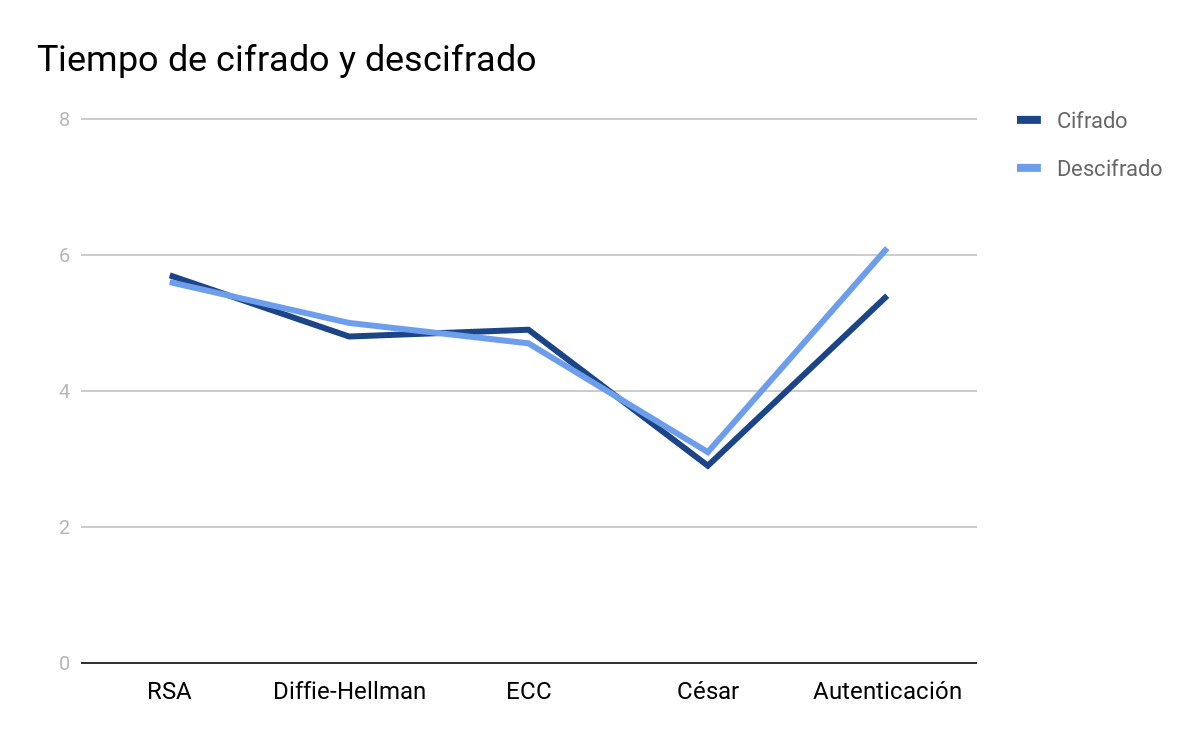
\includegraphics[width=6.27in,height=3.88in]{./media/image1.png}
	\end{Center}
\end{figure}


%%%%%%%%%%%%%%%%%%%% Figure/Image No: 2 Ends here %%%%%%%%%%%%%%%%%%%%

\par


\printbibliography
\end{document}